\documentclass{standalone}
\usepackage{tikz}
\usepackage{ctex,siunitx,ninecolors}
\setCJKmainfont{Noto Serif CJK SC}
\usepackage{tkz-euclide}
\usepackage{amsmath}
\usetikzlibrary{patterns, calc}
\usetikzlibrary {decorations.pathmorphing, decorations.pathreplacing, decorations.shapes,}
\begin{document}
\small
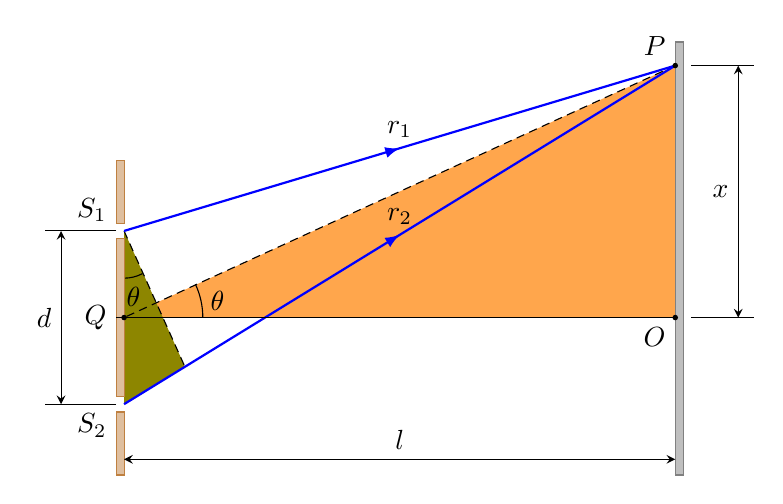
\begin{tikzpicture}[>=stealth,scale=1.0]
  \fill[orange!70](7,3.2)--(0,0)--(7,0);
  \fill[olive,opacity=50](0,1.1)--(0,-1.1)--(0.7728,-0.6253);
  \draw[densely dashed](7,3.2)--(0,0)(0,1.1)--(0.7728,-0.6253);
  \draw[thin](1.0,0)arc(0:25:1.0)node[midway,right]{$\theta$};
  \draw[thin](0,0.5)arc(270:298:0.5)node[midway,below]{$\theta$};
  \draw[brown,fill=brown!50](-0.1,1.0)rectangle(0,-1.0)(-0.1,1.2)rectangle(0,2)(-0.1,-1.2)rectangle(0,-2);
  \draw[gray,fill=lightgray](7,-2)rectangle(7.1,3.5);
  \draw[thin](-0.1,1.1)node[above left]{$S_1$}--(-1.0,1.1)(-0.1,-1.1)node[below left]{$S_2$}--(-1.0,-1.1);
  \draw[thick,blue,postaction={decorate},decoration={markings,mark=at position 0.5 with {\arrow{latex}}}](0,-1.1)--(7,3.2)node[midway,above,text=black]{$r_2$};
  \draw[thick,blue,postaction={decorate},decoration={markings,mark=at position 0.5 with {\arrow{latex}}}](0,1.1)--(7,3.2)node[midway,above,text=black]{$r_1$};
  \draw[thin](-0.1,0)node[left]{$Q$}--(7,0)node[below left]{$O$};
  \fill(0,0)circle(1pt)(7,0)circle(1pt)(7,3.2)circle(1pt)node[above left]{$P$};
  \draw[thin,<->](-0.8,-1.1)--(-0.8,1.1)node[midway,left]{$d$};
  \draw[thin](7.2,0)--(8,0)(7.2,3.2)--(8,3.2);
  \draw[thin,<->](7.8,0)--(7.8,3.2)node[midway,left]{$x$};
  \draw[thin,<->](0,-1.8)--(7,-1.8)node[midway,above]{$l$};
\end{tikzpicture}
\end{document}